\documentclass[convert=pdf2svg,multi=false]{standalone}
\usepackage{tikz}
  \usetikzlibrary{positioning}
\begin{document}
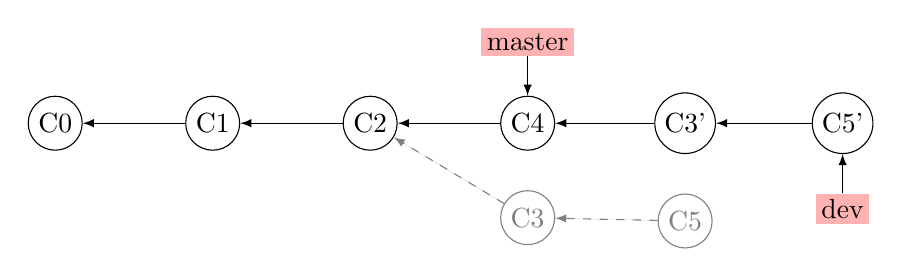
\begin{tikzpicture}[
  commit/.style={draw,circle,inner sep=2pt, minimum size=10pt},
  pointer/.style={draw=none,fill=red!30,rectangle,inner sep=2pt}]
\def\ancolor{black!50!white}
\tikzset{rebase/.style={commit, -latex, draw=\ancolor, text=\ancolor}}
\foreach \i[count=\x] in {0,1,2,4,3', 5'} {
   \node[commit] (C\i) at (2*\x,0) {C\i};
}
\node[rebase, below=.5 of C4] (C3) {C3};
\node[rebase, below=.5 of C3'] (C5) {C5};
\foreach \i/\j in {0/1,1/2,2/4,4/3',3'/5'} {
  \draw[latex-] (C\i) -- (C\j);
}
\draw[rebase, dashed, fill=\ancolor] (C5) -- (C3);
\draw[rebase, dashed, fill=\ancolor] (C3) -- (C2);
\node[pointer] (master) [above=.5 of C4] {master};
\node[pointer] (dev) [below=.5 of C5'] {dev};
\draw[-latex] (master) -- (C4);
\draw[-latex] (dev) -- (C5');
\end{tikzpicture}
\end{document}